% Poster (French): spruce budworm defoliation and Sentinel-1. Build: cd poster && lualatex poster_tbe_fr.tex
% Figures: TBE_AOI=saguenay_lsj python poster/poster_figures.py (from the repository root).
\documentclass[20pt,a0paper,portrait,margin=0mm,innermargin=18mm,blockverticalspace=14mm,colspace=16mm,subcolspace=8mm]{tikzposter}
\usepackage[french]{babel}
\usepackage{fontspec}
\setmainfont{TeX Gyre Heros}
\usepackage{graphicx,booktabs,xcolor,amsmath,enumitem,tabularx}
\usetikzlibrary{positioning,arrows.meta,fit,calc}
\usepackage[hidelinks]{hyperref}
\definecolor{accent}{HTML}{E08A00}
\definecolor{nuit}{HTML}{12304F}
\definecolor{radar}{HTML}{1F5FAE}
\definecolor{fond}{HTML}{F5F8FB}
\definecolor{gris}{HTML}{555555}
\usetheme{Simple}
\colorlet{backgroundcolor}{white}
\colorlet{framecolor}{white}
\colorlet{blocktitlebgcolor}{nuit}
\colorlet{blocktitlefgcolor}{white}
\colorlet{blockbodybgcolor}{fond}
\colorlet{blockbodyfgcolor}{black}
\colorlet{titlebgcolor}{white}
\colorlet{titlefgcolor}{nuit}
\defineblockstyle{Plat}{titlewidthscale=1, bodywidthscale=1, titleleft, titleoffsetx=0pt, titleoffsety=0pt,
  bodyoffsetx=0mm, bodyoffsety=12mm, bodyverticalshift=12mm, roundedcorners=6, linewidth=0pt,
  titleinnersep=9mm, bodyinnersep=11mm}{
  \draw[color=framecolor, fill=blockbodybgcolor, rounded corners=\blockroundedcorners] (blockbody.south west) rectangle (blockbody.north east);
  \ifBlockHasTitle
    \draw[color=framecolor, fill=blocktitlebgcolor, rounded corners=\blockroundedcorners] (blocktitle.south west) rectangle (blocktitle.north east);
  \fi}
\useblockstyle{Plat}
\setlist{leftmargin=1.1em,itemsep=4pt,topsep=4pt}
\newcommand{\Rb}[1]{\textcolor{radar}{\textbf{#1}}}
\newcounter{numfig}\newcounter{numtab}
\newcommand{\figcap}[1]{\stepcounter{numfig}{\small\textbf{Figure \thenumfig.} #1\par}\vspace{2mm}}
\newcommand{\tabcap}[1]{\stepcounter{numtab}{\small\textbf{Tableau \thenumtab.} #1\par}\vspace{1mm}}
\newcommand{\sous}[1]{\par\vspace{3mm}{\color{nuit}\large\bfseries #1\par}\vspace{1mm}}
\newcommand{\cle}[1]{\vspace{4mm}\colorbox{accent!14}{\parbox{0.97\linewidth}{\vspace{3mm}#1\vspace{3mm}}}\vspace{2mm}}

\settitle{
\begin{minipage}[c]{\linewidth}\centering
{\color{nuit}\fontsize{62}{74}\selectfont\bfseries La tordeuse des bourgeons de l'épinette vue par Sentinel-1\\[5mm]
\fontsize{46}{56}\selectfont un signal radar ouvert de la défoliation en forêt boréale québécoise\par}
\vspace{9mm}
{\fontsize{40}{48}\selectfont\color{black}\textbf{Mamadou Galy DIALLO}\par}
\vspace{3mm}
{\fontsize{30}{38}\selectfont\color{gris}galy.quantum@gmail.com\par}
\end{minipage}
\vspace{8mm}
{\color{accent}\rule{\linewidth}{5mm}}
}

\tikzposterlatexaffectionproofoff
\graphicspath{{figures/}}
\begin{document}
\maketitle[width=0.95\paperwidth, titletotopverticalspace=12mm, titletoblockverticalspace=10mm]

\begin{columns}
% ===================================================================== colonne gauche
\column{0.5}

\block{1. Introduction}{
Les épidémies de tordeuse des bourgeons de l'épinette (\textit{Choristoneura fumiferana}, TBE) défolient
périodiquement des millions d'hectares de sapinières et de pessières au Québec. Le ministère des Ressources
naturelles et des Forêts (MRNF) les cartographie chaque année par \textbf{relevé aérien} depuis 1967 : une
référence précise, mais coûteuse, dépendante de la météo et discontinue. Le radar \Rb{Sentinel-1} (bande C)
[1] est gratuit, acquis par tous les temps et revient tous les 6 à 12 jours sur toute la province.
\textbf{Ainsi, cette étude teste si des descripteurs radar ouverts, calculés uniquement avec des données
libres, portent un signal de la sévérité de la défoliation.}
\sous{Objectif}
Relier les composites estivaux Sentinel-1 de cinq étés (2017--2025) aux classes de sévérité du MRNF, puis
tester ce qui pourrait dépasser un simple indice : correction par pixel, texture, modèle physique et modèle
pré-entraîné sur Sentinel-1.
}

\block{2. Zone d'étude et données}{
\begin{minipage}[c]{0.55\linewidth}
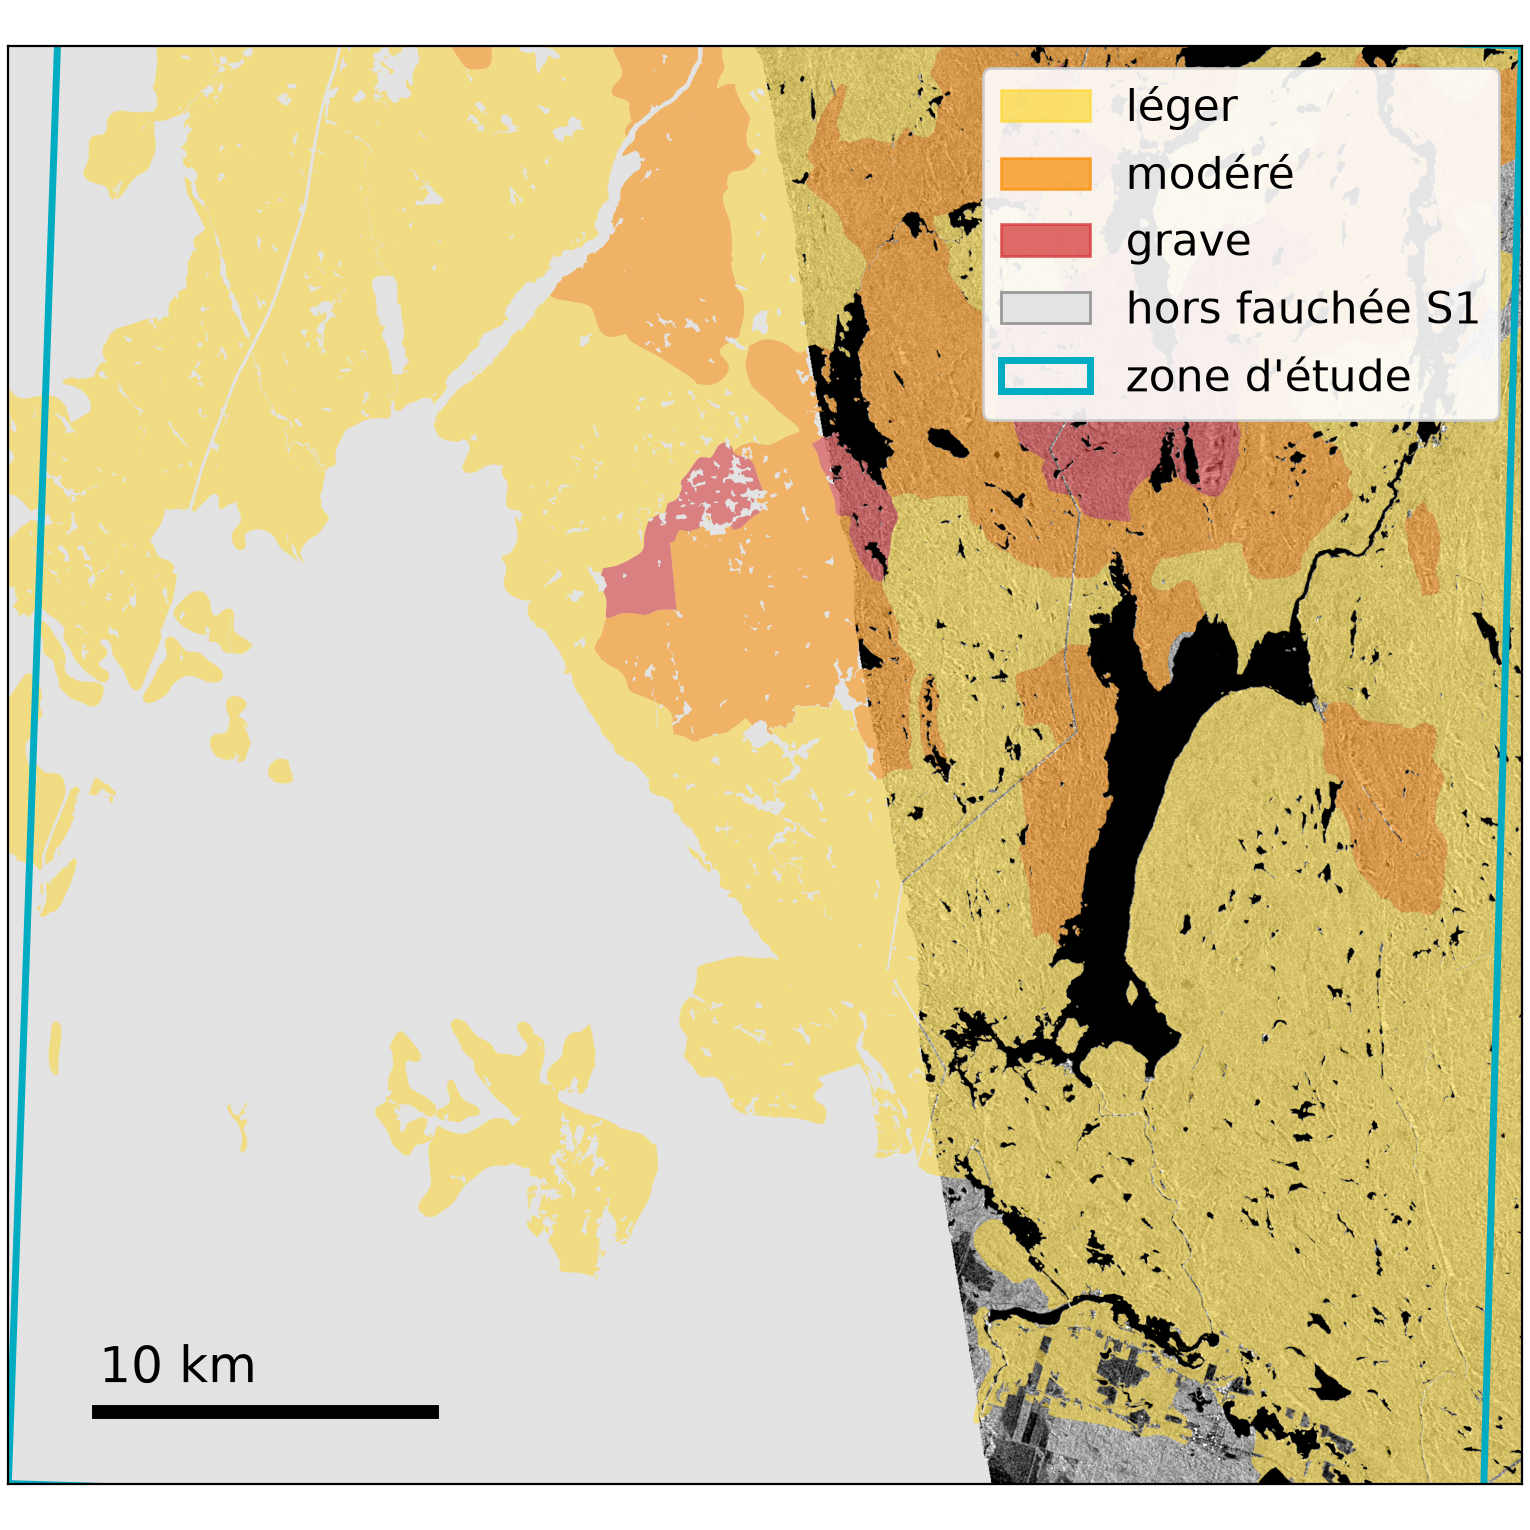
\includegraphics[width=\linewidth]{f0_carte.png}
\end{minipage}\hfill
\begin{minipage}[c]{0.42\linewidth}
\textbf{Saguenay--Lac-Saint-Jean} (1 961 km$^2$), épicentre de l'épidémie actuelle, retenu parmi quatre
régions pour la diversité de ses classes de sévérité.\par\vspace{3mm}
La fauchée Sentinel-1 de l'orbite retenue ne couvre qu'environ 45\,\% de la zone : seuls les polygones
qu'elle voit sont analysés.
\end{minipage}
\figcap{Sévérité de la défoliation en 2025 (relevé aérien MRNF) sur le composite Sentinel-1 VV de l'été 2025.}
\vspace{2mm}
\tabcap{Données, toutes en accès libre.}
\begin{center}\small
\begin{tabularx}{\linewidth}{@{}lX@{}}
\toprule
\Rb{Sentinel-1 RTC} & $\gamma^0$ VV, VH ; orbite relative 164 ; médiane des scènes du 15 juillet au 31 août ;
2017, 2019, 2021, 2023, 2025 ; grille de 20 m \\
Défoliation TBE & polygones annuels du MRNF (Données Québec, CC BY 4.0), classes léger, modéré, grave ;
témoins non affectés sur une grille de 1,5 km \\
Échantillons & 1 329 polygones (753 légers, 448 modérés, 91 graves, 37 non affectés) \\
Dendrochronologie & 3 chronologies ITRDB les plus proches (Krause et Morin) \\
\bottomrule
\end{tabularx}\end{center}
}

\block{3. Méthode}{
\begin{center}\resizebox{0.95\linewidth}{!}{%
\begin{tikzpicture}[font=\normalsize, node distance=9mm and 7mm,
  bx/.style={draw=nuit!70, fill=white, rounded corners=3mm, line width=1mm, align=center, minimum height=24mm},
  fl/.style={-{Latex[length=7mm,width=6mm]}, line width=1.4mm, nuit!70}]
\node[bx, draw=radar, fill=radar!8, text width=17cm] (s1) {\textbf{Sentinel-1 RTC} (Planetary Computer)\\ même orbite chaque année, composite médian};
\node[bx, text width=13cm, right=of s1] (mrnf) {\textbf{Polygones MRNF}\\ sévérité + témoins};
\node[bx, text width=32cm, below=14mm of $(s1.south)!0.5!(mrnf.south)$] (d) {\textbf{Paquet \texttt{nisar\_s1}} : composites, VV et VH en dB, RVI $= 4\,\mathrm{VH}/(\mathrm{VV}+\mathrm{VH})$ ;\\ statistiques zonales (moyenne, écart-type) par polygone};
\node[bx, fill=accent!14, text width=15cm, below=14mm of d.south west, anchor=north west] (a) {\textbf{Descripteurs}\\ forêt aléatoire, 5 plis, SHAP ;\\ anomalies, texture, Water Cloud Model};
\node[bx, fill=accent!14, text width=15cm, below=14mm of d.south east, anchor=north east] (b) {\textbf{Modèle pré-entraîné}\\ SSL4EO-S12 [4] sur Sentinel-1 ;\\ sonde linéaire, réglage fin};
\draw[fl] (s1.south) -- (s1.south|-d.north); \draw[fl] (mrnf.south) -- (mrnf.south|-d.north);
\draw[fl] (a.north|-d.south) -- (a.north); \draw[fl] (b.north|-d.south) -- (b.north);
\end{tikzpicture}}
\end{center}
\figcap{Schéma de la méthode. RVI : indice de végétation radar en double polarisation [2].}
}

\block{Références}{\footnotesize
\begin{enumerate}[label={[\arabic*]},leftmargin=2.1em,itemsep=2pt]
\item Torres \textit{et al.} (2012), \textit{Remote Sens. Environ.} 120, 9--24.
\item Kim \& van Zyl (2009), \textit{IEEE TGRS} 47, 2519--2527.
\item Attema \& Ulaby (1978), \textit{Radio Science} 13, 357--364.
\item Wang \textit{et al.} (2023), SSL4EO-S12, \textit{IEEE Geosci. Remote Sens. Mag.} 11, 98--106.
\end{enumerate}
\vspace{3mm}
{\color{gris}\textbf{Données} : Copernicus Sentinel-1 (ESA, UE) via Microsoft Planetary Computer ; défoliation
TBE © MRNF, Données Québec (CC BY 4.0) ; ITRDB (NOAA). \textbf{Code} : github.com/mamadou-g-diallo/sar-tbe-defoliation
et le paquet \texttt{nisar\_s1}.\par}
}

% ===================================================================== colonne droite
\column{0.5}

\block{4. Résultats}{
\sous{4.1 Le RVI détecte la défoliation, mais ne la gradue pas}
\begin{minipage}[c]{0.5\linewidth}
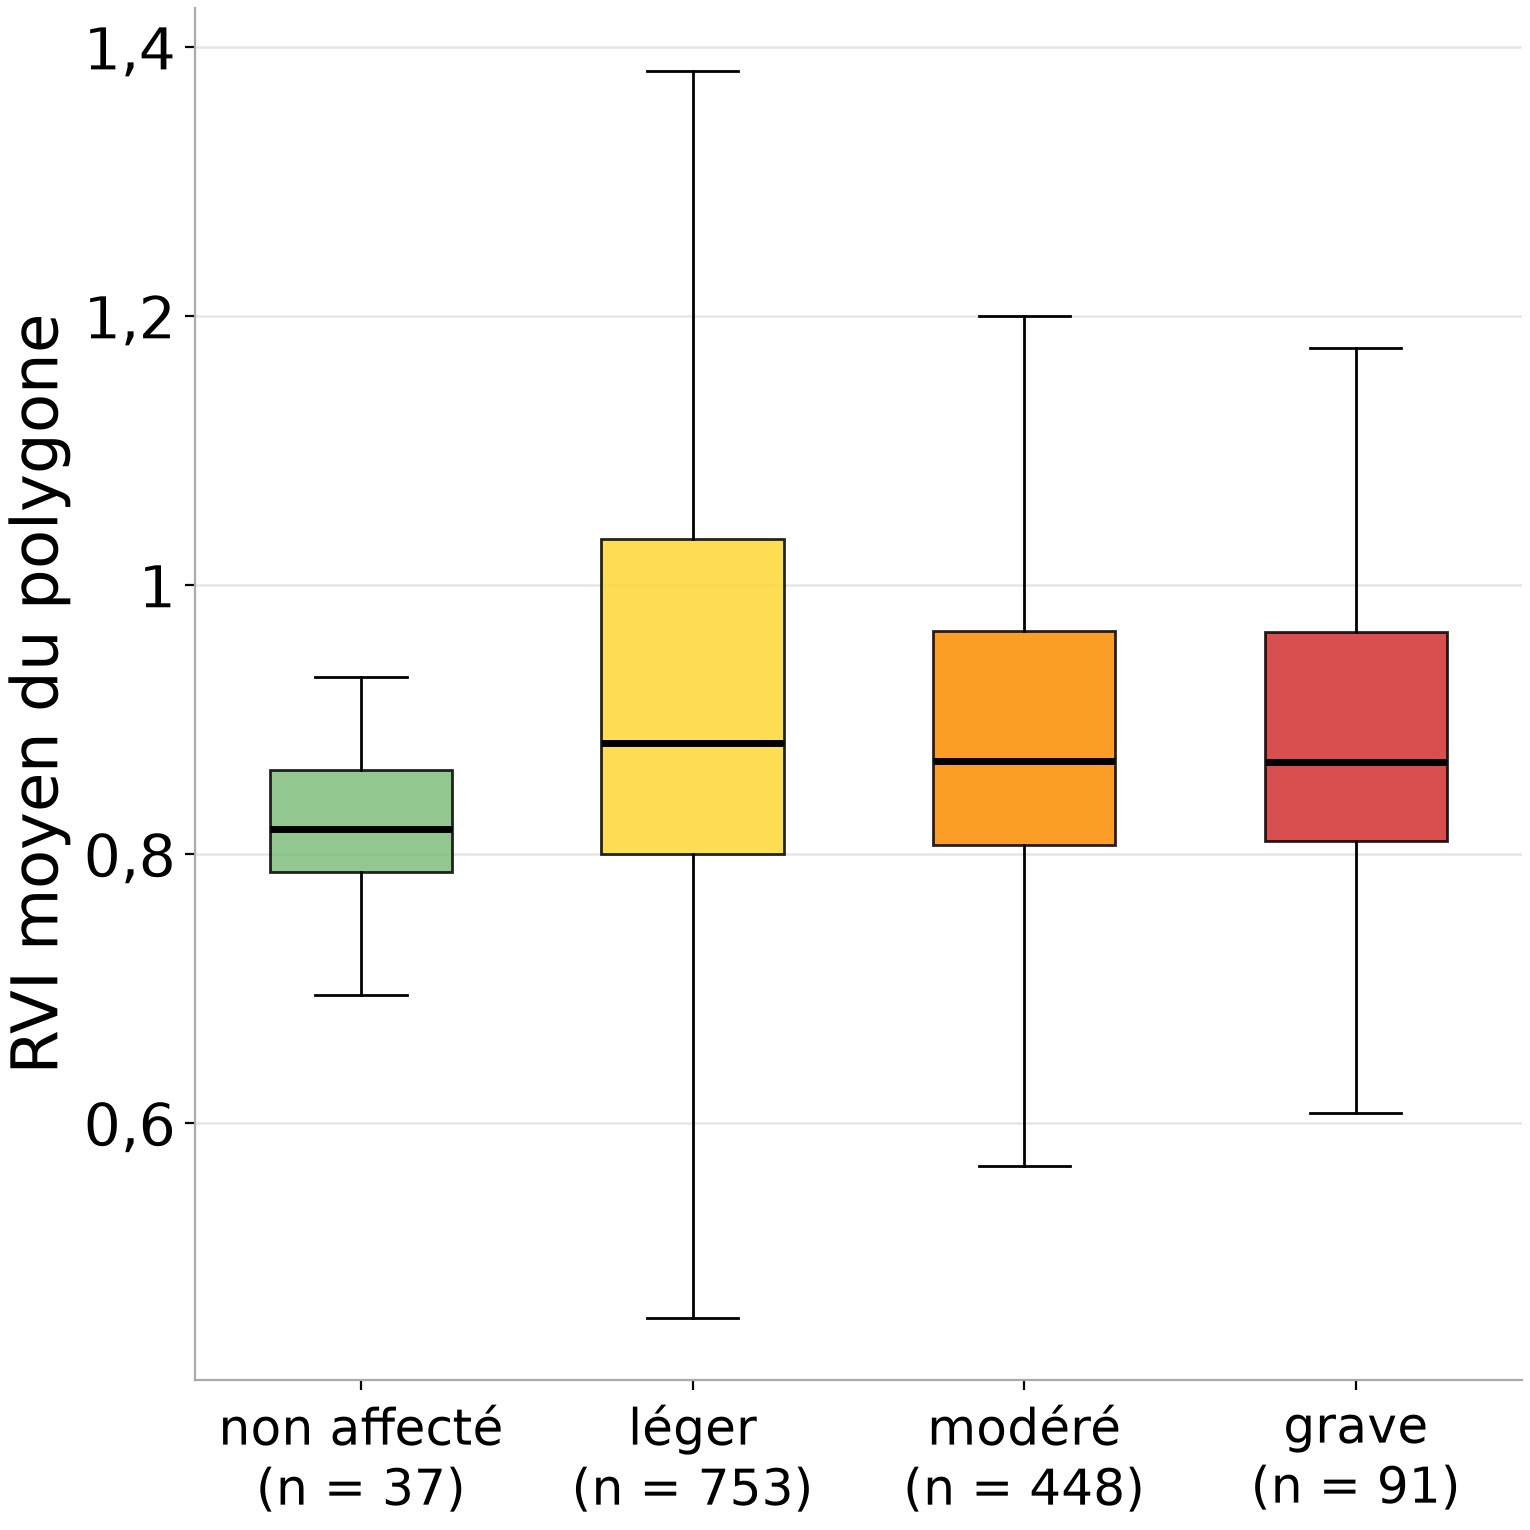
\includegraphics[width=\linewidth]{f1_rvi.png}
\end{minipage}\hfill
\begin{minipage}[c]{0.47\linewidth}
Les témoins non affectés se regroupent autour d'un RVI de \textbf{0,82} ; toute défoliation donne un RVI plus
élevé et plus dispersé (médianes \textbf{0,87--0,88}). Les trois classes de sévérité se recouvrent
largement. SHAP place la \textbf{variabilité intra-polygone} du RVI avant sa moyenne.
\end{minipage}
\figcap{RVI moyen par polygone selon la classe de sévérité (boîtes : quartiles ; moustaches : 1,5 fois
l'écart interquartile).}

\sous{4.2 Un modèle pré-entraîné gradue mieux la sévérité}
\begin{minipage}[c]{0.5\linewidth}
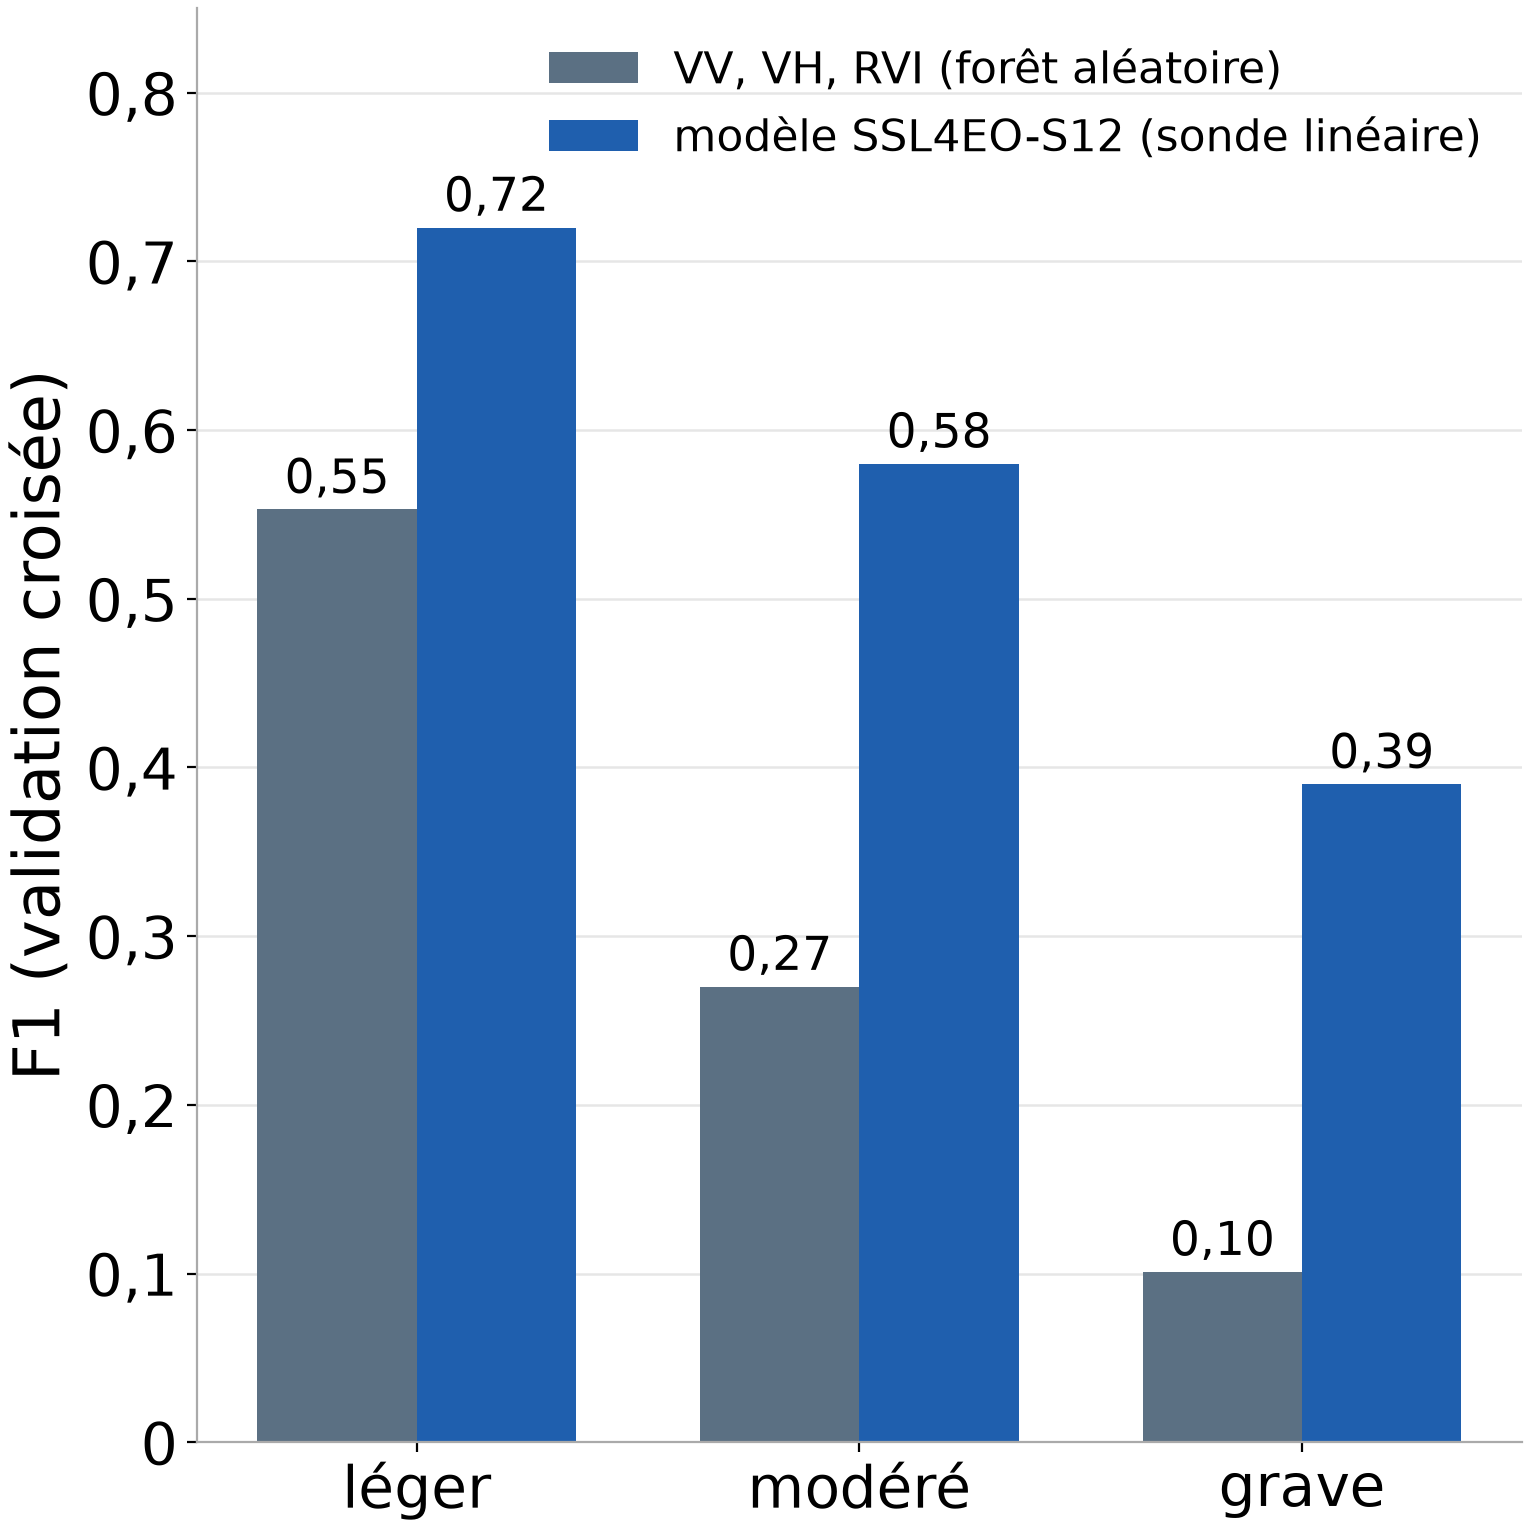
\includegraphics[width=\linewidth]{f2_f1.png}
\end{minipage}\hfill
\begin{minipage}[c]{0.47\linewidth}
\tabcap{Exactitude de la forêt aléatoire (5 plis).}
{\small\setlength{\tabcolsep}{6pt}
\begin{tabular}{@{}lr@{}}
\toprule
VV, VH, RVI & 0,38 \\
anomalies par pixel & 0,41 \\
texture GLCM ($n$ = 431) & 0,35 \\
amplitude + texture & 0,40 \\
\Rb{SSL4EO-S12, sonde} & \Rb{0,64} \\
SSL4EO-S12, réglage fin$^*$ & 0,60 \\
\bottomrule
\end{tabular}}\\[1mm]
{\footnotesize $^*$ un seul jeu de test, $n$ = 212.}
\end{minipage}
\figcap{F1 par classe de sévérité : descripteurs d'amplitude contre plongements du modèle SSL4EO-S12.}
\cle{Aucun descripteur construit à la main ne dépasse \textbf{0,41} d'exactitude ; le modèle pré-entraîné
atteint \Rb{0,64} et relève surtout les classes difficiles : F1 \Rb{0,58} contre 0,27 pour « modéré »,
\Rb{0,39} contre 0,10 pour « grave ». La classe « léger » représentant 57\,\% des échantillons, ce sont ces
F1 par classe, et non l'exactitude globale, qui mesurent le gain.}

\sous{4.3 Ce que les tests négatifs apprennent}
\begin{itemize}
\item \textbf{Water Cloud Model} [3] à angle unique : R$^2$ négatif ; sans angle d'incidence local ni
humidité mesurée, le modèle physique n'explique rien.
\item \textbf{Bord de fauchée} : 8\,\% des pixels, près du bord, sont sous $-$30 dB (bruit) ; masquer une
bande de 2 km change peu le résultat (0,41 contre 0,38 ; F1 « modéré » 0,28 contre 0,27).
\item \textbf{Dendrochronologie} : les chronologies ouvertes captent l'épidémie de 1978, mais s'arrêtent en
1993--1995, avant Sentinel-1.
\end{itemize}
}

\block{5. Discussion et conclusions}{
Cette étude teste, sur données ouvertes uniquement, si Sentinel-1 porte un signal de la défoliation par la
tordeuse. Le RVI \textbf{détecte} la défoliation mais ne la \textbf{gradue} pas, et aucun descripteur
construit à la main ne dépasse 0,41 d'exactitude : le plafond ne tient pas à un descripteur manquant, mais
à l'information physique absente (angle d'incidence local, eau du houppier, mesures de terrain). Un modèle
pré-entraîné sur Sentinel-1 améliore nettement les classes modérée et grave, ce qui montre que l'information
existe dans les images. Ces résultats restent limités : une seule région, une fauchée partielle, une
référence issue de relevés aériens. \textbf{Ainsi, en perspective}, la cohérence interférométrique, la
bande L (NISAR, puis ROSE-L), des mesures de terrain couplées à un modèle physique et le transfert du modèle
pré-entraîné à d'autres régions sont des pistes à explorer.
}

\end{columns}
\end{document}
